This file contains the annotations to be stamped into the pdf.
A note consists of the page number of the note, the position of the
annotations on the page and the annotation itself.
Everything outside the tags <begin:foo> and <end:foo> will be ignored.


If there are any packages you might need to include on the note generation,
enter them between the <begin:packages> and <end:packages> tags.
Default packages are amsmath, amssymb, textpos, geometry and color.
Be sure to also include their configurations, if needed.
<begin:packages>
\usepackage{tikz}
<end:packages>


The first line should have: PAGE, WIDTH, XPOSITION, YPOSITION.
PAGE should be one number. WIDTH, XPOSITION and YPOSITION should be a number appended of a LaTeX unit (except ex and em). 
Everything after that, until the <end:note> tag will be considered the note itself.

Common margins:
Letter (left) : PAGE, 1.75cm, 0.1cm, YPOSITION
Letter (right): PAGE, 1.45cm, 19.7cm, YPOSITION
A4     (left) : PAGE, 1.75cm, 0.1cm, YPOSITION 
A4     (right): PAGE, 1.45cm, 19cm, YPOSITION 
B4     (left) : PAGE, 1.75cm, 0.1cm, YPOSITION 
B4     (right): PAGE, 1.45cm, 23.05cm, YPOSITION 

<begin:note>
1, 2.1cm, 0.1cm, 11.2cm
\tiny Tiny ``lorem ipsum dolor si amet'' and a script-sized equation: \\
\scriptsize
\[\int_{\mathbb{R}} e^{-t^2} \, dt = \sqrt{\pi}\]
<end:note>

<begin:note>
1, 2.0cm, 18.7cm, 3in
\scriptsize From $\sin(\pi) = 0$, we can conclude that no integers $x$, $y$, $z$
can satisfy: \[x^n + y^n = z^n\] for any $n > 2$.
<end:note>

<begin:note>
1, 15cm, 18cm, 0.1cm
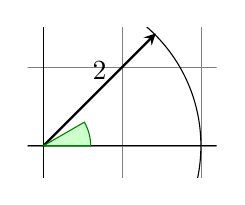
\begin{tikzpicture}[scale=2,>=stealth]
    \clip (-0.1,-0.2) rectangle (1.1,0.75);
    \draw[step=.5cm,gray,very thin] (-1.4,-1.4) grid (1.4,1.4);
    \draw (-1.5,0) -- (1.5,0);
    \draw (0,-1.5) -- (0,1.5);
    \draw (0,0) circle (1cm);
    \draw[->,thick] (0,0) -- (0.713,0.713) node[midway,anchor=south] {2};
    \filldraw[fill=green!20!white, draw=green!50!black]
        (0,0) -- (3mm,0mm) arc (0:30:3mm) -- cycle;
\end{tikzpicture}
<end:note>
